
\section{Release Notes}

The purpose of ESMF v1.0 is to provide a first look at the ESMF
Application Programming Interface (API), and to demonstrate the viability 
of the ESMF architecture and implementation.  For this release, we have focused 
on implementing major architectural features and basic functionality.  The 
current performance characteristics and memory requirements of the software 
are unlikely to resemble those in later releases.  

We are relying on Earth system modelers to provide us with the feedback necessary 
to realize this goal.  Section \ref{sec:Support} of this document includes 
instructions on submitting comments on ESMF v1.0 to our development team.

Our next major release, ESMF v2.0, will occur in April 2004.  At that time, 
the {\it ESMF User's Guide} will be expanded to include a comprehensive section 
on how to adapt application codes for the framework, and support staff will be 
available to assist users with ESMF adoption.  We anticipate, but have 
not scheduled, other public releases and patches between now and ESMF v2.0.  
Our focus during this year will be on developing an easy to use, production-quality 
product.  

\section{What is the Earth System Modeling Framework?}

The Earth System Modeling Framework (ESMF) is a structured collection of 
software building blocks that can be used or customized to develop 
Earth system model components, and assemble them into applications.  
The simplest view of the ESMF is that it consists of an {\it infrastructure} 
of utilities and data structures for creating 
model components, and a {\it superstructure} for coupling them.  
User code sits between these two layers, making calls to the infrastructure
libraries beneath it and being scheduled and synchronized by the 
superstructure above it.  The configuration resembles a sandwich, as
shown in Figure~\ref{fig:TheESMFwich}.

The ESMF architecture is scalable, flexible paradigm for building highly 
complex climate, weather, and related applications from components such
as atmospheric models, land models, and data assimilation systems.  The 
ESMF is not a single master application into which all components must fit; 
rather it is a way of developing components so that they can be used 
in many different user-written applications.  Model components that adopt 
ESMF are usable in different contexts without code modification, and may be
incorporated into other ESMF-based modeling systems within the Earth 
science community.  In addition to high-level organization, ESMF provides 
a set of robust, portable, performance optimized libraries for regridding, 
data transfers, I/O, time management, and other common modeling functions.  
ESMF users may choose to extensively rewrite their codes to take advantage 
of the ESMF infrastructure, or they may decide to simply wrap user-written 
components in ESMF interfaces in order to adopt the ESMF architecture and 
utilize framework coupling services.

\section{The ESMF User's Guide}

This {\it ESMF User's Guide} will eventually serve as an introduction for the 
new ESMF user and as a reference for the experienced user.  Since ESMF 
Release 1.0 is the first public ESMF release, and is a prototype rather than 
a production-ready package, we assume you are a potential user interested in 
learning more about the ESMF software.  This edition of the {\it User's Guide} 
is designed to guide you through that process.  We strongly encourage you
to download the ESMF software and try running a demonstration program, 
{\tt ESMF\_COUPLED\_FLOW}, that illustrates both ESMF utilities and coupling
services.

The next two sections, \ref{sec:Support} and \ref{sec:Submission}, concern 
user support and how to submit comments on the ESMF system to our develoment 
team.  Section \ref{sec:QuickStart} contains a {\it Quick Start} guide that 
explains how to install the ESMF software and 
run the demonstration program.  Section \ref{sec:ArchOver} is an 
architectural overview that describes the framework's basic goals and features.The next few Sections, beginning with \ref~{sec:demo}, describe in detail
the {\tt ESMF\_COUPLED\_FLOW} demo application.    
More detail on ESMF structure and operation, such as a description of the 
directory structure and how to run the ESMF self-tests, is provided in Section 
\ref{sec:TechOver}.  Section \ref{sec:Adoption} looks ahead to the steps 
required to adapt a component for use with ESMF.  Finally, to help you become 
familiar with ESMF terminology, the last section in the {\it User's Guide} is 
a glossary.  

\begin{center}
\begin{figure}
\caption{Schematic of ESMF ``sandwich'' architecture. In this design the framework consists of two parts. An upper level
{\bf Superstructure} layer and a lower-level {\bf Infrastructure} layer. User code is sandwiched between these two layers.}
\label{fig:TheESMFwich}
\scalebox{1.0}{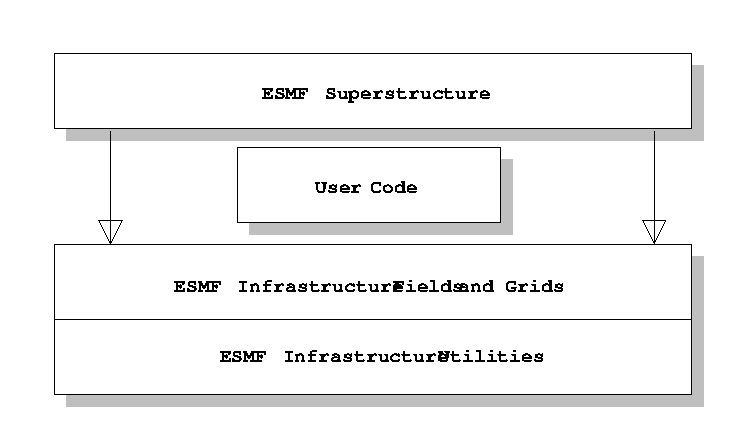
\includegraphics{esmfwich.EPS}}
\end{figure}
\end{center}
















